\documentclass{ximera}

 

\usepackage{epsfig}

\graphicspath{
  {./}
  {figures/}
}

\usepackage{morewrites}
\makeatletter
\newcommand\subfile[1]{%
\renewcommand{\input}[1]{}%
\begingroup\skip@preamble\otherinput{#1}\endgroup\par\vspace{\topsep}
\let\input\otherinput}
\makeatother

\newcommand{\includeexercises}{\directlua{dofile("/home/jim/linearAlgebra/laode/exercises.lua")}}

%\newcounter{ccounter}
%\setcounter{ccounter}{1}
%\newcommand{\Chapter}[1]{\setcounter{chapter}{\arabic{ccounter}}\chapter{#1}\addtocounter{ccounter}{1}}

%\newcommand{\section}[1]{\section{#1}\setcounter{thm}{0}\setcounter{equation}{0}}

%\renewcommand{\theequation}{\arabic{chapter}.\arabic{section}.\arabic{equation}}
%\renewcommand{\thefigure}{\arabic{chapter}.\arabic{figure}}
%\renewcommand{\thetable}{\arabic{chapter}.\arabic{table}}

%\newcommand{\Sec}[2]{\section{#1}\markright{\arabic{ccounter}.\arabic{section}.#2}\setcounter{equation}{0}\setcounter{thm}{0}\setcounter{figure}{0}}

\newcommand{\Sec}[2]{\section{#1}}

\setcounter{secnumdepth}{2}
%\setcounter{secnumdepth}{1} 

%\newcounter{THM}
%\renewcommand{\theTHM}{\arabic{chapter}.\arabic{section}}

\newcommand{\trademark}{{R\!\!\!\!\!\bigcirc}}
%\newtheorem{exercise}{}

\newcommand{\dfield}{{\sf dfield9}}
\newcommand{\pplane}{{\sf pplane9}}

\newcommand{\EXER}{\section*{Exercises}}%\vspace*{0.2in}\hrule\small\setcounter{exercise}{0}}
\newcommand{\CEXER}{}%\vspace{0.08in}\begin{center}Computer Exercises\end{center}}
\newcommand{\TEXER}{} %\vspace{0.08in}\begin{center}Hand Exercises\end{center}}
\newcommand{\AEXER}{} %\vspace{0.08in}\begin{center}Hand Exercises\end{center}}

% BADBAD: \newcommand{\Bbb}{\bf}

\newcommand{\R}{\mbox{$\Bbb{R}$}}
\newcommand{\C}{\mbox{$\Bbb{C}$}}
\newcommand{\Z}{\mbox{$\Bbb{Z}$}}
\newcommand{\N}{\mbox{$\Bbb{N}$}}
\newcommand{\D}{\mbox{{\bf D}}}
\usepackage{amssymb}
%\newcommand{\qed}{\hfill\mbox{\raggedright$\square$} \vspace{1ex}}
%\newcommand{\proof}{\noindent {\bf Proof:} \hspace{0.1in}}

\newcommand{\setmin}{\;\mbox{--}\;}
\newcommand{\Matlab}{{M\small{AT\-LAB}} }
\newcommand{\Matlabp}{{M\small{AT\-LAB}}}
\newcommand{\computer}{\Matlab Instructions}
\newcommand{\half}{\mbox{$\frac{1}{2}$}}
\newcommand{\compose}{\raisebox{.15ex}{\mbox{{\scriptsize$\circ$}}}}
\newcommand{\AND}{\quad\mbox{and}\quad}
\newcommand{\vect}[2]{\left(\begin{array}{c} #1_1 \\ \vdots \\
 #1_{#2}\end{array}\right)}
\newcommand{\mattwo}[4]{\left(\begin{array}{rr} #1 & #2\\ #3
&#4\end{array}\right)}
\newcommand{\mattwoc}[4]{\left(\begin{array}{cc} #1 & #2\\ #3
&#4\end{array}\right)}
\newcommand{\vectwo}[2]{\left(\begin{array}{r} #1 \\ #2\end{array}\right)}
\newcommand{\vectwoc}[2]{\left(\begin{array}{c} #1 \\ #2\end{array}\right)}

\newcommand{\ignore}[1]{}


\newcommand{\inv}{^{-1}}
\newcommand{\CC}{{\cal C}}
\newcommand{\CCone}{\CC^1}
\newcommand{\Span}{{\rm span}}
\newcommand{\rank}{{\rm rank}}
\newcommand{\trace}{{\rm tr}}
\newcommand{\RE}{{\rm Re}}
\newcommand{\IM}{{\rm Im}}
\newcommand{\nulls}{{\rm null\;space}}

\newcommand{\dps}{\displaystyle}
\newcommand{\arraystart}{\renewcommand{\arraystretch}{1.8}}
\newcommand{\arrayfinish}{\renewcommand{\arraystretch}{1.2}}
\newcommand{\Start}[1]{\vspace{0.08in}\noindent {\bf Section~\ref{#1}}}
\newcommand{\exer}[1]{\noindent {\bf \ref{#1}}}
\newcommand{\ans}{}
\newcommand{\matthree}[9]{\left(\begin{array}{rrr} #1 & #2 & #3 \\ #4 & #5 & #6
\\ #7 & #8 & #9\end{array}\right)}
\newcommand{\cvectwo}[2]{\left(\begin{array}{c} #1 \\ #2\end{array}\right)}
\newcommand{\cmatthree}[9]{\left(\begin{array}{ccc} #1 & #2 & #3 \\ #4 & #5 &
#6 \\ #7 & #8 & #9\end{array}\right)}
\newcommand{\vecthree}[3]{\left(\begin{array}{r} #1 \\ #2 \\
#3\end{array}\right)}
\newcommand{\cvecthree}[3]{\left(\begin{array}{c} #1 \\ #2 \\
#3\end{array}\right)}
\newcommand{\cmattwo}[4]{\left(\begin{array}{cc} #1 & #2\\ #3
&#4\end{array}\right)}

\newcommand{\Matrix}[1]{\ensuremath{\left(\begin{array}{rrrrrrrrrrrrrrrrrr} #1 \end{array}\right)}}

\newcommand{\Matrixc}[1]{\ensuremath{\left(\begin{array}{cccccccccccc} #1 \end{array}\right)}}



\renewcommand{\labelenumi}{\theenumi)}
\newenvironment{enumeratea}%
{\begingroup
 \renewcommand{\theenumi}{\alph{enumi}}
 \renewcommand{\labelenumi}{(\theenumi)}
 \begin{enumerate}}
 {\end{enumerate}\endgroup}



\newcounter{help}
\renewcommand{\thehelp}{\thesection.\arabic{equation}}

%\newenvironment{equation*}%
%{\renewcommand\endequation{\eqno (\theequation)* $$}%
%   \begin{equation}}%
%   {\end{equation}\renewcommand\endequation{\eqno \@eqnnum
%$$\global\@ignoretrue}}

%\input{psfig.tex}

\author{Martin Golubitsky and Michael Dellnitz}

%\newenvironment{matlabEquation}%
%{\renewcommand\endequation{\eqno (\theequation*) $$}%
%   \begin{equation}}%
%   {\end{equation}\renewcommand\endequation{\eqno \@eqnnum
% $$\global\@ignoretrue}}

\newcommand{\soln}{\textbf{Solution:} }
\newcommand{\exercap}[1]{\centerline{Figure~\ref{#1}}}
\newcommand{\exercaptwo}[1]{\centerline{Figure~\ref{#1}a\hspace{2.1in}
Figure~\ref{#1}b}}
\newcommand{\exercapthree}[1]{\centerline{Figure~\ref{#1}a\hspace{1.2in}
Figure~\ref{#1}b\hspace{1.2in}Figure~\ref{#1}c}}
\newcommand{\para}{\hspace{0.4in}}

\renewenvironment{solution}{\suppress}{\endsuppress}

\ifxake
\newenvironment{matlabEquation}{\begin{equation}}{\end{equation}}
\else
\newenvironment{matlabEquation}%
{\let\oldtheequation\theequation\renewcommand{\theequation}{\oldtheequation*}\begin{equation}}%
  {\end{equation}\let\theequation\oldtheequation}
\fi

\makeatother


\title{Introduction}

\begin{document}
\begin{abstract}
\end{abstract}
\maketitle


\label{S:introAPNS}

In Section~\ref{S:PSP&E} we discussed phase line pictures of 
a single autonomous\index{differential equation!autonomous} 
differential equation 
\index{phase!line}
\[
\frac{dx}{dt} = f(x).
\]
We saw that knowing the equilibria\index{equilibrium} and the dynamics 
near those equilibria was sufficient information for understanding 
the dynamics of all solutions.  For example, if 
\begin{equation}  \label{e:1dexample}
f(x) = x(x-1)(x-2)=x^3-3x^2+2x,
\end{equation}
then the differential equation has three equilibria located at 
$0,1$, and $2$.  From the derivative
\[
f'(x)=3x^2-6x+2
\]
we see that 
\[
f'(0)=2, \quad f'(1)=-1, \AND f'(2)=2.
\]
So the equilibria at $x=0$ and $x=2$ are unstable\index{unstable} 
(since the derivative 
is positive at these equilibria) while the equilibrium at $1$ is 
asymptotically stable (since the derivative is negative at $x=1$). 
\index{stability!asymptotic} 
Recall Theorem~\ref{T:stability1} of Chapter~\ref{chap:SolveOdes}.  
This information is summarized in the phase line picture in 
Figure~\ref{F:pp1d}.

\begin{figure}[htb]
           \centerline{%
            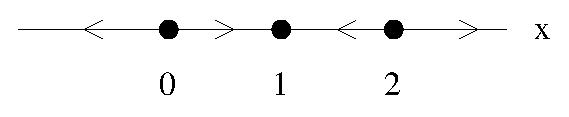
\psfig{file=../figures/pp1d.eps,height=0.6in}}
           \caption{Phase line plot for the one dimensional equation
	\protect\eqref{e:1dexample}.}
           \label{F:pp1d}
\end{figure}

The added content of Figure~\ref{F:pp1d} is that we now know the 
fate of all solutions in both forward and backward time.  A 
solution $x(t)$ with initial condition at $x_0$ between the 
equilibria $0$ and $1$ approaches $1$ in forward time
($t\to\infty$) and $0$ in backward time ($t\to -\infty$).  
This information is 
encoded in the arrows on the figure.  Using {\dfield}
\index{\computer!dfield8} we can 
find the time series of \eqref{e:1dexample} for an initial condition 
between $0$ and $1$.  See Figure~\ref{F:pp1dt}. Alternatively, this  
phase line tells us the equilibria and the trajectories that connect 
equilibria.  If we assume a finite number of equilibria and that the
derivative is nonzero at each equilibrium, then in one dimension 
there is nothing else that can happen in the dynamics.

\begin{figure}[htb]
           \centerline{%
            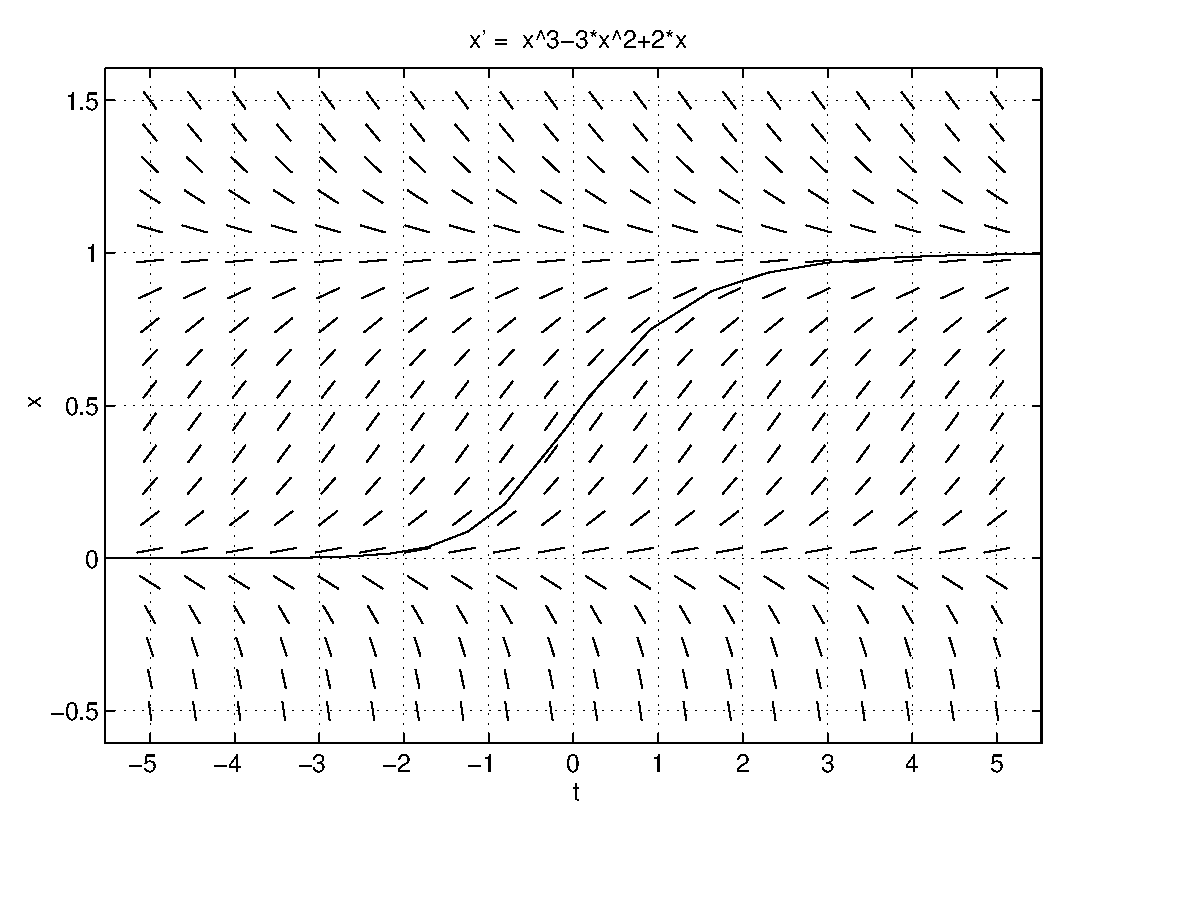
\psfig{file=../figures/pp1dt.eps,height=2.0in}}
           \caption{Time series for solution to \protect\eqref{e:1dexample}
	with initial condition between $0$ and $1$.}
           \label{F:pp1dt}
\end{figure}





\subsection*{Two Dimensional Phase Planes}

The purpose of this chapter is to develop a similar understanding 
of phase portraits for two dimensional autonomous systems
\arraystart
\begin{equation} \label{e:nonlinear2}
\begin{array}{rcl} 
\dps\frac{dx}{dt} & = & f(x,y) \\
\dps\frac{dy}{dt} & = & g(x,y).
\end{array}
\end{equation}
As is the case in one dimension, equilibria and trajectories 
connecting these equilibria play a major role in determining  
phase portraits.  In two dimensions, however, there is a new 
type of solution that also plays a role in determining phase 
plane pictures: the periodic solution\index{periodic solution}.  
The remainder of this 
introduction illustrates the type of information that we will 
want to include in two dimensional phase portraits. \index{phase!plane}

\subsubsection*{A Linear Equation}

In Section~\ref{S:PlanarSystems} we saw that the dynamics of planar
constant coefficient linear differential equations are determined by the 
eigenvalues and eigenvectors of the coefficient matrix.  We  
review some of this material in Section~\ref{S:linearization}. 
For example, the origin\index{origin} is a saddle\index{saddle}
in the system of differential equations
\begin{matlabEquation}  \label{e:localexam}
\begin{array}{rcl} 
\dps\frac{dx}{dt} & = & y \\
\dps\frac{dy}{dt} & = & 2.2x+2.1y 
\end{array}
\end{matlabEquation}
\arrayfinish
\noindent {\bf Note:} The * after the label \eqref{e:localexam} indicates 
that this differential equation has been preloaded in the file {\tt 
e11\_1\_3.pps} and can be addressed from {\pplane}
\index{\computer!pplane8} by clicking sequentially on the 
{\sf File} button in the {\sf PPLANE8 Setup} window, the 
{\sf Load a system from...} button, and the {\tt laode toolbox} button.  
Then click on the {\tt e11\_1\_3.pps} file and the {\sf Done} button to 
load the differential equation \eqref{e:localexam} into {\pplane}.

The fact that the origin in \eqref{e:localexam} is a saddle is seen by 
examining the coefficient matrix of \eqref{e:localexam}
\[
C = \mattwo{0}{1}{2.2}{2.1}.
\]
Note that $\det(C)=-2.2<0$.  Since the determinant is the product 
of the eigenvalues, the eigenvalues of $C$ are real and of opposite 
sign; and the origin is a saddle.  See Table~\ref{T:hyperbolic} in 
Section~\ref{S:PlanarSystems}.

Using \Matlab we can determine more refined information
concerning the dynamics of this equation.  The two eigenvalues
of $C$ are found by entering $C$ and typing {\tt eig(C)}
to obtain
\begin{verbatim}
ans = 
   -0.7673
    2.8673
\end{verbatim}
thus verifying that the eigenvalues are real and of opposite
sign.  Moreover, we can find the eigenvectors\index{eigenvector}
\index{eigenvalue} associated with these eigenvalues by typing
\begin{verbatim}
[V,D] = eig(C)
\end{verbatim}\index{\computer!eig}
to obtain
\begin{verbatim}
V = 
   -0.7934   -0.3293
    0.6087   -0.9442
 
D =
   -0.7673         0
         0    2.8673
\end{verbatim} 
The eigenvectors are the columns of the matrix $V$ and this 
information allows us to sketch the dynamics of
\eqref{e:localexam} as in Figure~\ref{F:local} (left).  Indeed, we
can use {\pplane} to plot more accurately the phase plane
picture associated to \eqref{e:localexam}, as shown in
Figure~\ref{F:local} (right).  Note also that the eigenvalue and eigenvector
information is determined in {\pplane}.  In the {\sf PPLANE8 Display}
window click on the {\sf solutions} button and then on the {\sf Find an 
equilibrium} button.  Use the cross hairs to click near the origin.  Then 
{\pplane} finds the equilibrium and shows the matrix $C$ and its eigenvalues
and eigenvectors in the {\sf PPLANE8 Equilibrium point data} window.

\begin{figure*}[htb]
           \centerline{%
           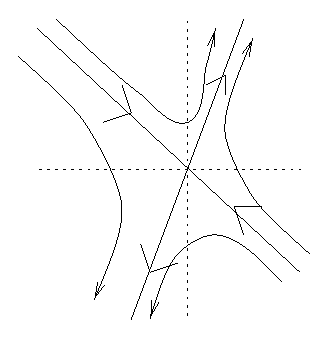
\psfig{file=../figures/locala.eps,height=1.8in}
           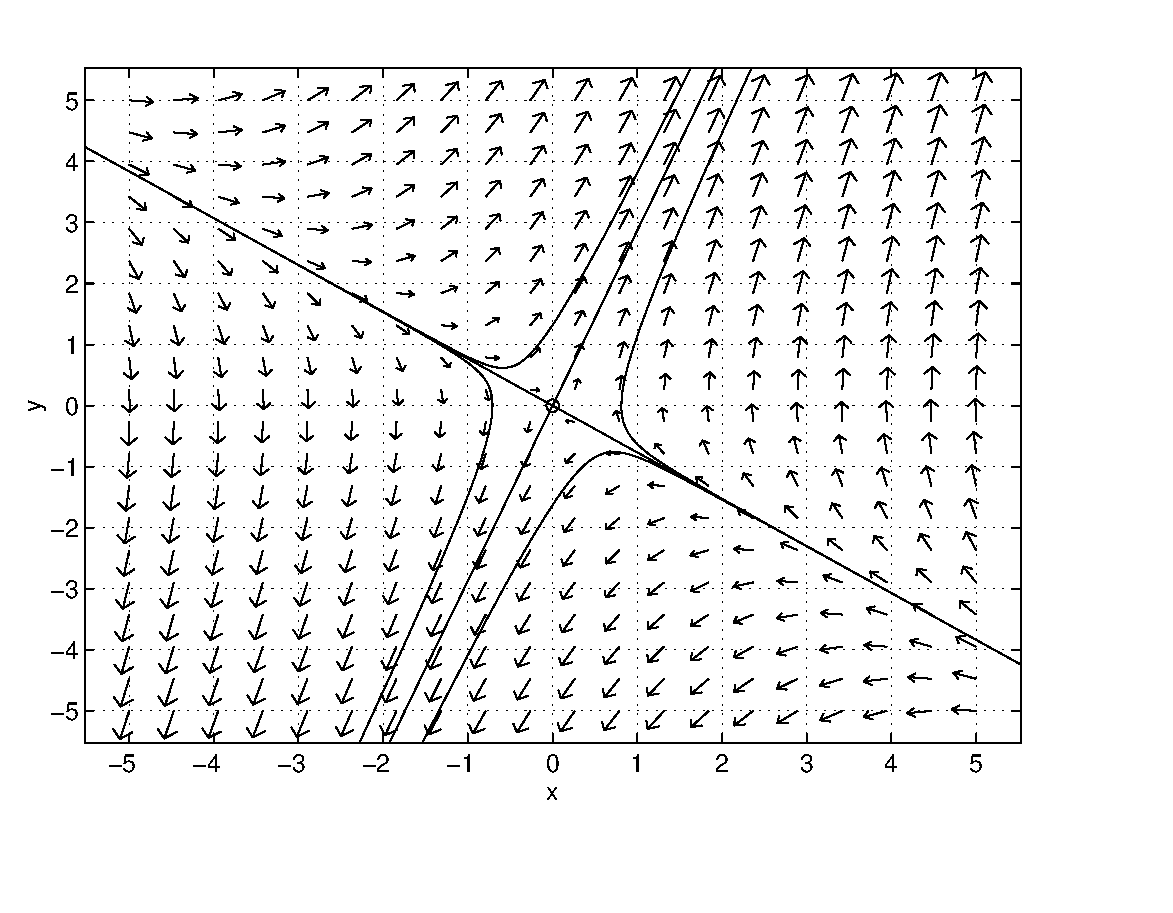
\psfig{file=../figures/localb.eps,height=2.0in}}
           \caption{(Left) Sketch of phase plane of \protect\eqref{e:localexam} 
	based on eigenvalues and eigenvectors of $C$. (Right) Trajectories 
	of \protect\eqref{e:localexam} using {\pplane}.}
           \label{F:local}
\end{figure*}

\subsubsection*{The Addition of Nonlinear Terms}
 
Next we discuss what happens to solutions when nonlinear terms are added to 
\eqref{e:localexam}.  For example, consider the system
\index{nonlinear!system of differential equations}
\index{differential equation!nonlinear}
\arraystart
\begin{matlabEquation}  \label{e:globalexam}
\begin{array}{rcl} 
\dps\frac{dx}{dt} & = & y \\
\dps\frac{dy}{dt} & = & 2.2x+2.1y +x^2+xy. 
\end{array}
\end{matlabEquation}
\arrayfinish
We study the phase plane of \eqref{e:globalexam} using {\pplane} and find 
that trajectories\index{trajectory} for the nonlinear system on the square 
$-0.5\leq x,y \leq 0.5$ look very much like those for the linear system 
\eqref{e:localexam} --- even though we do not know how to solve the nonlinear
system in closed form, as we can for the linear system. See 
Figure~\ref{F:globala} and note the similarity of this figure with 
Figure~\ref{F:local} (right).
\begin{figure}[hbt]
           \centerline{%
           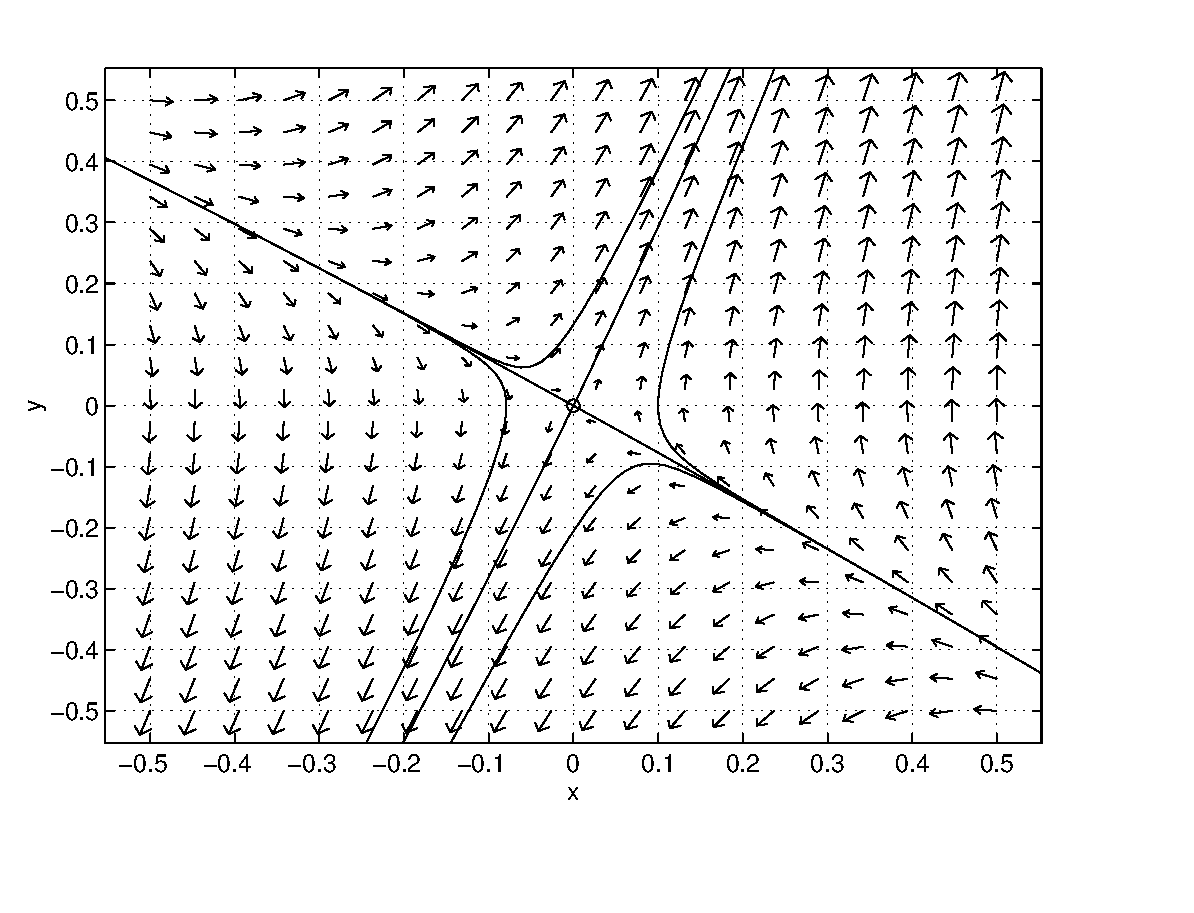
\psfig{file=../figures/globala.eps,height=2.0in}}
           \caption{Trajectories of \protect\eqref{e:globalexam} 
	on the square $-0.5\leq x,y \leq 0.5$ using {\pplane}.}
           \label{F:globala}
\end{figure}

Recall that an equilibrium is {\em hyperbolic\/} \index{hyperbolic} 
if the eigenvalues of
the matrix of coefficients of the linear terms have nonzero real 
part.  There is a theorem that states that in a sufficiently small
neighborhood of a hyperbolic equilibrium of a nonlinear system,
the trajectories {\em look like\/} the solutions of the
associated linear system.  Indeed, on the small square in which
these numerical calculations were performed, this theorem appears
to be correct.

However, when we compute the solution trajectories to
\eqref{e:globalexam} on the larger square $-5\leq x,y\leq 5$, it
becomes clear that the phase plane\index{phase!plane} picture of 
the nonlinear
system no longer resembles the phase plane picture of the linear
system.  See Figure~\ref{F:globalb} (left).
\begin{figure*}[htb]
           \centerline{%
	   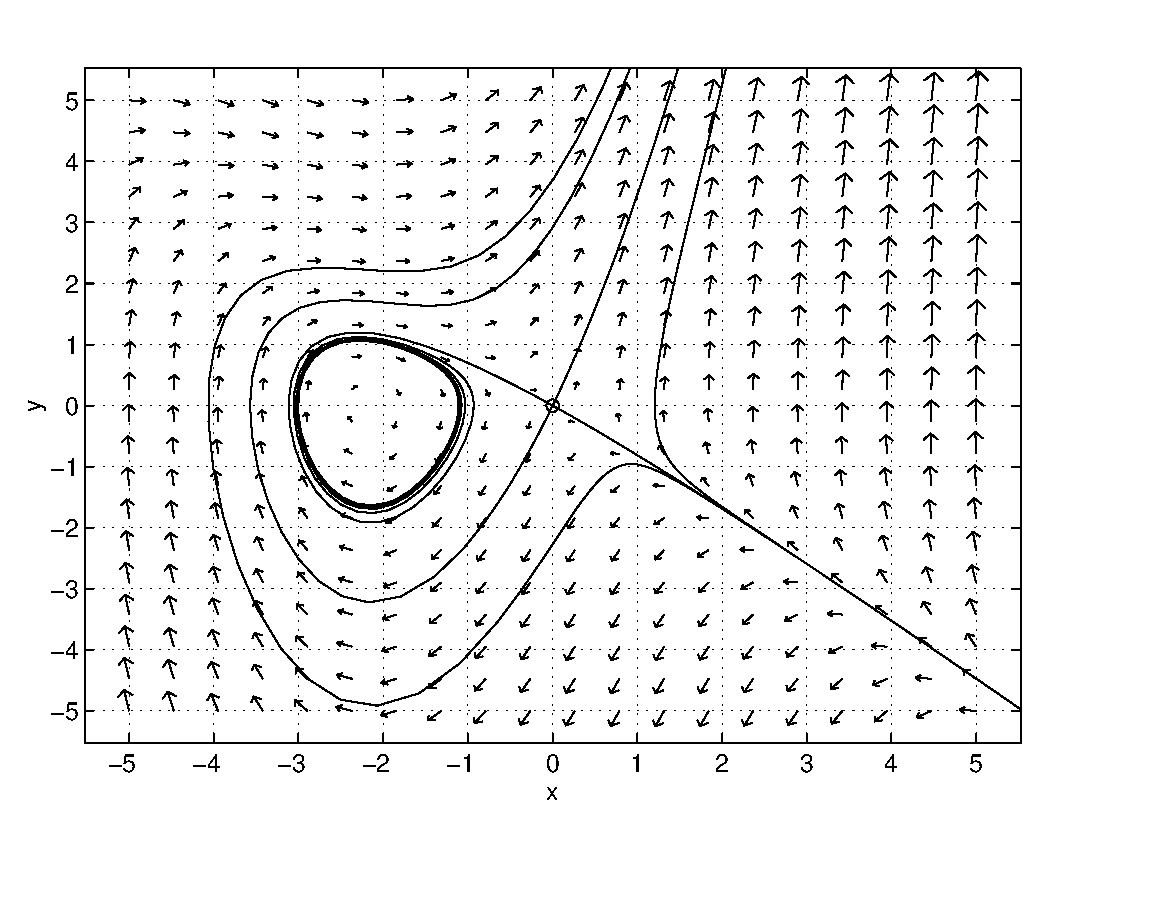
\psfig{file=../figures/globalb.eps,height=2.0in}
           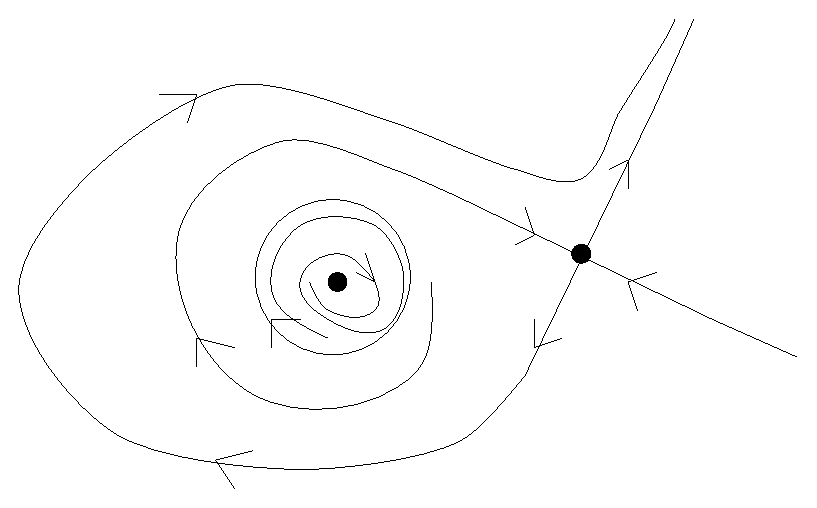
\psfig{file=../figures/globalc.eps,height=2.0in}}
           \caption{(Left) Trajectories of \protect\eqref{e:globalexam} 
on the square $-5\leq x,y \leq 5$ using {\pplane}. (Right) A
phase plane portrait of this equation.}
           \label{F:globalb}
\end{figure*}
Note that there is another equilibrium, a spiral sink\index{sink},
surrounded by what looks like a circular trajectory.  In 
Figure~\ref{F:globalb} (right) we sketch a phase portrait for 
this system of ODEs indicating the important information: 
the equilibria and type of equilibria, the periodic solutions,
\index{periodic solution}
and the connections between these trajectories.  Note that we have found
these trajectories numerically even though we do not know how to solve for
them in closed form.

\subsubsection*{The Importance of Phase Plane Portraits}

The importance of the phase portrait is that it lets us determine the 
evolution of solutions starting in the square --- even though we do not 
have a formula for these solutions.  For example, we can use 
{\sf Keyboard input} to start a trajectory near the origin so
that its backward evolution
approaches the periodic solution
while its forward evolution leaves the square in the unstable
direction\index{unstable!direction} of the saddle\index{saddle} at 
the origin.  In Figure~\ref{F:nltraj}
we picture the trajectory in phase space through the point 
$(-0.1,0.1)$, along with the time series $y$ versus $t$ of this
solution.  

\begin{figure*}[htb]
           \centerline{%
	   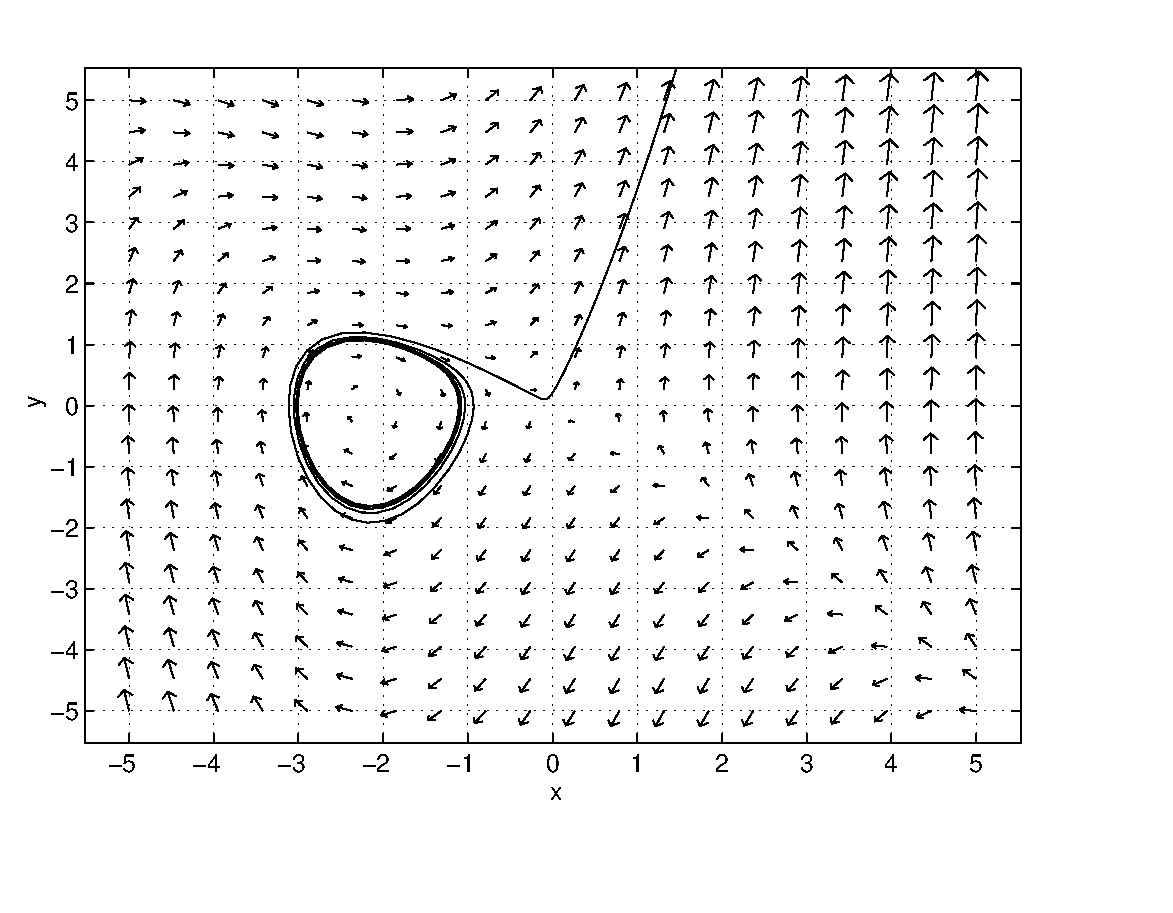
\psfig{file=../figures/nltraj.eps,height=2.5in}
           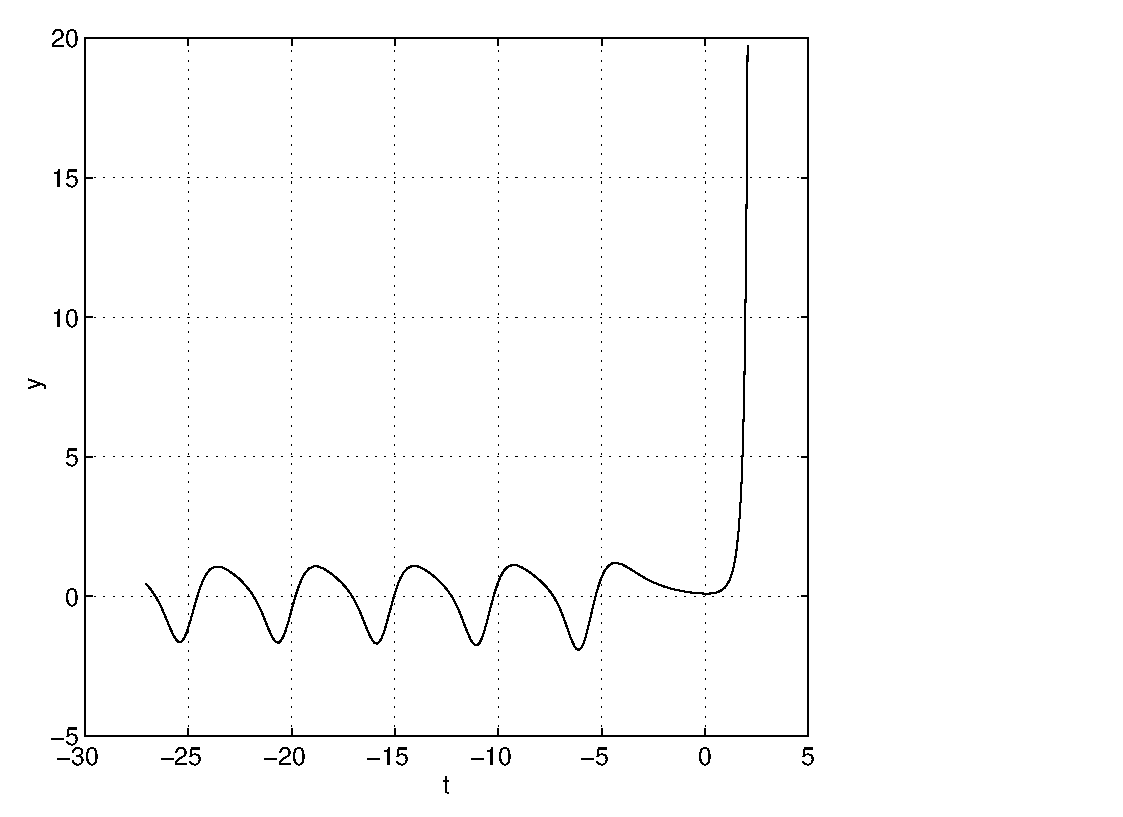
\psfig{file=../figures/nlts.eps,height=2.0in}}
           \caption{(Left) Trajectory of \protect\eqref{e:globalexam} 
	through $(-0.1,0.1)$. (Right) Time series $y$ versus $t$ of
this solution.}
           \label{F:nltraj}
\end{figure*}


In this chapter we discuss what kinds of dynamics we can expect
from autonomous planar systems of differential equations.  We 
show that solutions to linear systems give us much 
information about the structure of solutions to nonlinear 
systems.  We also show that there are new phenomena 
occurring in solutions to nonlinear systems that do not occur 
in solutions to the linear ones.  In our discussions we abandon 
any attempts at proofs; rather we try to survey the most 
important theorems with an eye to understanding how they can 
help with numerical explorations.

\EXER

\includeexercises




\end{document}
